\subsection{Role within the VO architecture}
 The IVOA Provenance Data Model is adding metadata to trace the orignal process followed during the data production to provide astronomical data. Even if it borrows the main general concepts defined in the data management science, it binds to the specific context of astronomical metadata description and re-uses or interacts with existing IVOA models.
It takes benefits from existing IVOA notations and standards like UCD, VOUnits, VO protocols and service design and is planned for a full integration into the VO landscape.

\TODO{Will be inserted later.}
% Skipping this for now. Let's not let this draft look more official than it 
% currently is.

\begin{figure}
\centering
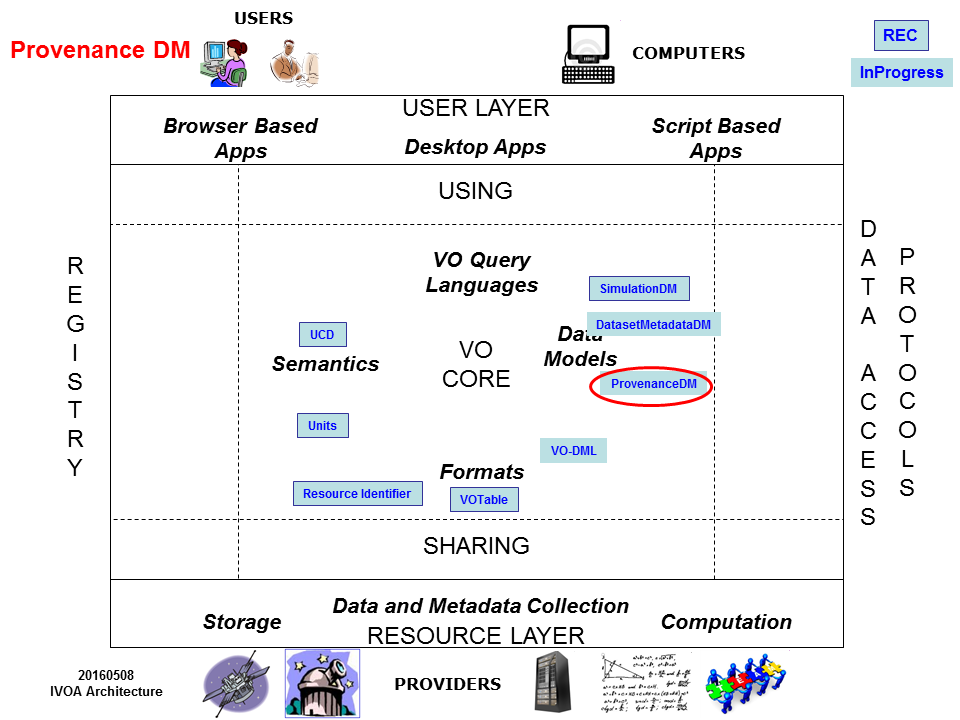
\includegraphics[width=0.9\textwidth]{VOArchitecture-Prov2016.png}
\caption{Architecture diagram for the Provenance Data model. It is based on existing concepts defined in existing IVOA data models, and existing formats and semantics and fully integrated in the IVOA framework}
\label{fig:archdiag}
\end{figure}

Fig.~\ref{fig:archdiag} shows the dependencies of this document with respect to other existing standards.
%IVOA architecture \citep{note:VOARCH}.
